
\chapter{Introdução}
\label{cap:intro}

O controle adaptativo é uma área em sistemas de controle, que busca projetar controladores capazes de se ajustarem automaticamente às mudanças e incertezas presentes no ambiente \cite{controle_adaptativo_livro}. Essa abordagem é especialmente relevante em cenários complexos, onde o conhecimento prévio do modelo do sistema se torna insuficiente para garantir um desempenho satisfatório. Sabendo que o intuito principal de controles adaptativos está na estimativa dos valores dos parâmetros, para que esta abordagem seja aplicada em um ambiente incerto é necessário ser feita uma análise bem abrangente, levando em consideração todos os pontos que podem gerar incertezas, até que encontre o estimador adequado, sendo que este pode se tornar obsoleto ao passar do tempo, caso o problema mude drasticamente suas características.

Nesse contexto, a utilização do Aprendizado por Reforço (Reinforcement Learning - RL) como ferramenta para o controle adaptativo tem ganhado destaque \cite{ac_rl_intersections}. O RL permite que um agente aprenda a tomar decisões por meio de interações com um ambiente, buscando maximizar a recompensa acumulada ao longo do tempo \cite{sutton}. Com o RL, o agente pode aprender políticas que se adaptem às mudanças do ambiente e melhorem seu desempenho de forma contínua.

Alguns contextos se mostram mais desafiadores que outros e dificultam o processo de busca por soluções satisfatórias. Quando a situação requer uma ação e esta possui resultados imediatos, isso se mostra um contexto mais simples do que aquele onde as ações tomadas no instante atual só terão implicações em um horizonte de tempo mais distante, as chamadas tarefas de Longo Horizonte (Long-Horizon). Resolver este tipo de tarefa ainda é um desafio e está sendo explorado \cite{dream_v1}, \cite{dreamer_v2}. Existem algumas abordagens que fazem uso das características presentes em RL para auxiliar na solução de tarefas Long-Horizon \cite{relay_long_horizon}, \cite{dream_v1}, \cite{dremaer_v3}. 

Futebol de robôs é um ambiente de estratégias e de aprimoramento constante. Neste trabalho destaca-se uma categoria específica, que aborda este tema, dentro da Competição Brasileira de Robótica - CBR, Very Small Size Soccer - VSSS \cite{regras_vss2023}. O futebol de robôs é um contexto que reúne características atrativas para testes e experimentações acerca do tema em estudo, pois é um ambiente que permite a modelagem por meio de RL \cite{bruno_brandao}, necessita de controle para realizar o deslocamento apropriado dos robôs \cite{trabalho_thiago} e utiliza de imagens como feedback das trajetórias \cite{regras_vss2023}. Neste sentido, o emprego de soluções que se propõe a resolverem tarefas de longo horizonte e soluções que utilizam RL para auxiliar em controle se mostra promissor, visto que é um contexto que envolve estratégias e mudanças constantes. 

O objetivo desta pesquisa é explorar o uso do algoritmo Dreamer \cite{dream_v1} para desenvolver um sistema de Controle Adaptativo aplicado ao contexto do futebol de robôs. O Dreamer é um algoritmo que fornece um agente capaz de aprender comportamentos de longo horizonte a partir de imagens somente pela imaginação latente \cite{dream_v1} ilustrado na Figura \ref{fig:resumo_dreamer}. Imaginação latente é a habilidade que um modelo tem de criar novos exemplos ou amostras que extrapolam os dados de treinamento, usando uma representação de baixa dimensionalidade chamada espaço latente \cite{dream_v1}.

\begin{figure}[H]
 \centering
 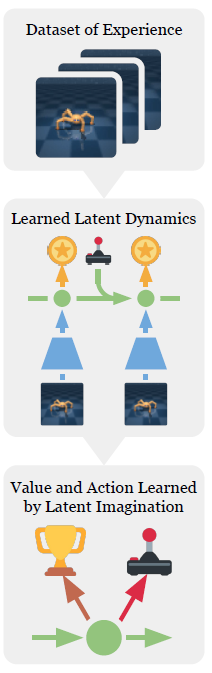
\includegraphics[width=0.20\textwidth]{./fig/resumo_dreamer.png}

 \caption{Dreamer aprende um modelo de mundo a partir de experiências passadas e aprende com eficiência comportamentos presentes em seu espaço latente, retro propagando estimativas de valor por meio de trajetórias imaginadas.
 Fonte: \cite{dream_v1}}
 \label{fig:resumo_dreamer}
\end{figure}